%% Standalone figure for the Statistical Mechanics exercises (Quiz 1).
%% Build: pdflatex quiz1_agpr.tex  (or run build.sh in this folder)
\documentclass[11pt,tikz,border=2pt]{standalone}
\usepackage{amsmath,amssymb}
\usetikzlibrary{arrows.meta, positioning}
\begin{document}
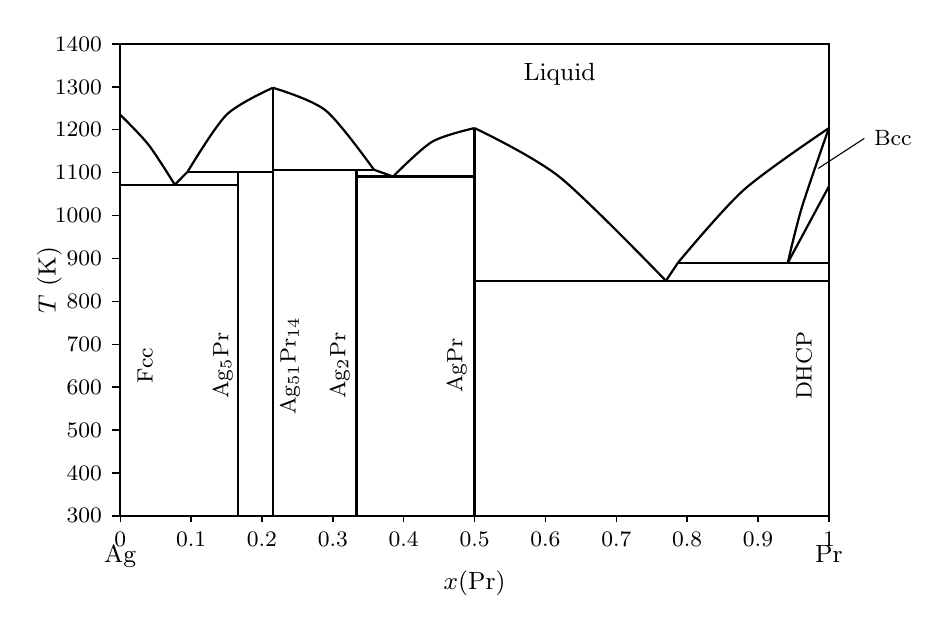
\begin{tikzpicture}[font=\small, >=Latex, line width=0.8pt]
\begin{scope}[x=9cm, y=0.0054545cm, shift={(0,-300)}]
    % frame and ticks
    \draw (0,300) rectangle (1,1400);
    \foreach \T in {300,400,...,1400}
        \draw[line width=0.5pt] (0,\T) -- (-0.012,\T) node[left, font=\footnotesize] {\T};
    \foreach \x/\l in {0/0,0.1/0.1,0.2/0.2,0.3/0.3,0.4/0.4,0.5/0.5,0.6/0.6,0.7/0.7,0.8/0.8,0.9/0.9,1/1}
        \draw[line width=0.5pt] (\x,300) -- (\x,285) node[below, font=\footnotesize] {\l};
    % liquidus
    \draw plot[smooth] coordinates {(0,1235) (0.04,1165) (0.077,1072)};
    \draw (0.077,1072) -- (0.095,1102);
    \draw plot[smooth] coordinates {(0.095,1102) (0.15,1235) (0.2154,1298)};
    \draw plot[smooth] coordinates {(0.2154,1298) (0.29,1245) (0.358,1107)};
    \draw (0.358,1107) -- (0.385,1091);
    \draw plot[smooth] coordinates {(0.385,1091) (0.44,1172) (0.5,1204)};
    \draw plot[smooth] coordinates {(0.5,1204) (0.62,1090) (0.770,848)};
    \draw (0.770,848) -- (0.787,890);
    \draw plot[smooth] coordinates {(0.787,890) (0.88,1060) (1.0,1204)};
    % Bcc solidus and Bcc/DHCP boundary
    \draw plot[smooth] coordinates {(1.0,1204) (0.962,1020) (0.942,890)};
    \draw (0.942,890) -- (1.0,1068);
    % three-phase isotherms
    \draw (0,1072) -- (0.1667,1072);
    \draw (0.095,1102) -- (0.2154,1102);
    \draw (0.2154,1107) -- (0.358,1107);
    \draw (0.3333,1091) -- (0.5,1091);
    \draw (0.5,848) -- (1.0,848);
    \draw (0.787,890) -- (1.0,890);
    % stoichiometric compounds
    \draw (0.1667,300) -- (0.1667,1102);
    \draw (0.2154,300) -- (0.2154,1298);
    \draw (0.3333,300) -- (0.3333,1107);
    \draw (0.5,300) -- (0.5,1204);
    % phase labels
    \node at (0.62,1330) {Liquid};
    \draw[line width=0.4pt] (0.985,1110) -- (1.05,1180) node[right, font=\footnotesize] {Bcc};
    \begin{scope}[font=\footnotesize]
        \node[rotate=90] at (0.035,650) {Fcc};
        \node[rotate=90] at (0.145,650) {Ag$_5$Pr};
        \node[rotate=90] at (0.240,650) {Ag$_{51}$Pr$_{14}$};
        \node[rotate=90] at (0.310,650) {Ag$_2$Pr};
        \node[rotate=90] at (0.475,650) {AgPr};
        \node[rotate=90] at (0.965,650) {DHCP};
    \end{scope}
    % axis labels
    \node[below=16pt] at (0.5,300) {$x$(Pr)};
    \node[below=4pt] at (0,280) {Ag};
    \node[below=4pt] at (1,280) {Pr};
    \node[rotate=90] at (-0.10,850) {$T$ (K)};
\end{scope}
\end{tikzpicture}
\end{document}
